\documentclass[12pt]{article}
\usepackage{graphicx}
\usepackage{multirow}
\usepackage{minted}
\usepackage{hyperref}
\setminted{fontsize=\footnotesize}
\usepackage{hyperref}

\title{High-performance Computing, Autumn 2024}
\author{Robert Buj}
\date{\today}

\begin{document}
\maketitle

\section*{Question 1}

The graph below shows the execution time of the parallel implementation (OpenMP) of the sum of the different elements of the vector $a$ ($sum = \sum_{n=0}^{N-1} a_i$) using the reduction clause. sum time means $T_{PAR}$ and, global time means $T_{PAR}+T_{SEQ}$. To simplify the source code, the last two sentences that should be part of $T_{PAR}$ are omitted.

\begin{figure}[h!]
	\centering
	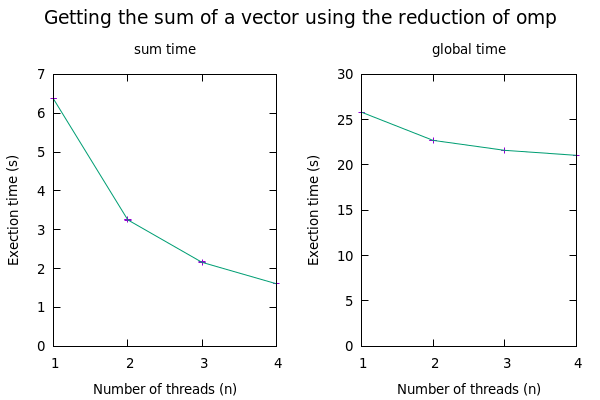
\includegraphics[width=0.8\linewidth]{sv.png}
	\caption{Execution time for adding 1000000000 elements}
	\label{fig:reduction}
\end{figure}

\newpage

\begin{figure}[h!]
	\inputminted{c}{sv.c}
	\caption{sv.c}\label{code:sv}
\end{figure}

\newpage

\section*{Question 2}

In the figures below, you can see the execution times of the multiplication of two matrices. The Figure~\ref{fig:mm} summarizes the execution time for mm, and the Figure~\ref{fig:mm2} summarizes the execution time for mm2.

\begin{figure}[h!]
	\centering
	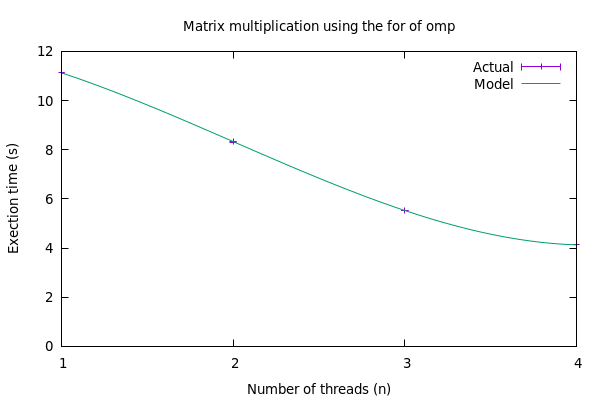
\includegraphics[width=0.7\linewidth]{mm.png}
	\caption{Execution time of mm}
	\label{fig:mm}
\end{figure}

\begin{figure}[h!]
	\centering
	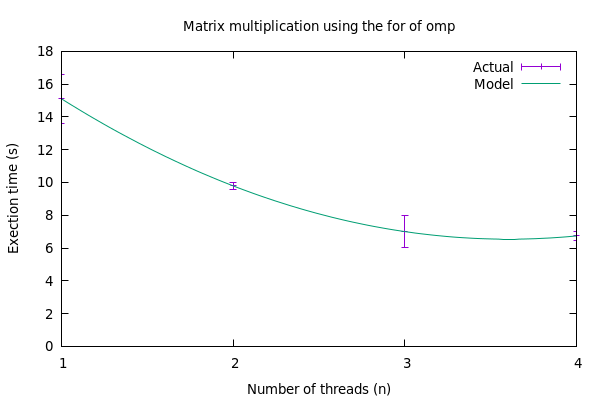
\includegraphics[width=0.7\linewidth]{mm2.png}
	\caption{Execution time of mm2}
	\label{fig:mm2}
\end{figure}

\newpage

\begin{figure}[h!]
	\inputminted{c}{mm.c}
	\caption{mm.c}\label{code:mmomp}
\end{figure}

\newpage

\begin{figure}[h!]
	\inputminted{c}{mm2.c}
	\caption{mm2.c}\label{code:mm2omp}
\end{figure}

\newpage

\section*{Question 3}

In the second file there are more cache misses. On each iteration or very frequently, the data block that contains the element mresult[i][j] has to be loaded from main memory to cache as well as matrix[i][k], and then the result has to be stored from cache to memory (mresult[i][j]), and that has a time penalty. The deeper loop changes the value of i all time (j*i*k times), it means that it changes the row of the matrices mresult and matrix, which is not a consecutive memory position, thus it can't be found on existing stored data in cache and hence the cache miss.

\begin{table}[h!]
	\centering
\begin{tabular}{|l|r|r|c|}
	\hline
	& flops & flops2 & factor \\
	\hline
	Real\_time & 11.158243 & 13.867895 & 1.24 \\
	\hline
	Proc\_time & 11.1389094 & 13.8486805 & 1.24 \\
	\hline
	Total\_flpins & 2000768595 & 2003602758 & = \\
	\hline
	MFLOPS & 179.6227218 & 145.9744919 & 0.81 \\
	\hline
\end{tabular}
	\caption{Resume of flops.}
\label{tab:flopsresume}
\end{table}

\begin{table}[h!]
	\centering
	\begin{tabular}{|l|l|l|l|l|}
		\hline
		host & Real\_time & Proc\_time & Total\_flpins & MFLOPS \\
		\hline
		compute-0-0.local & 11.086303 & 11.060439 & 2000306880 & 180.852402 \\
		compute-0-1.local & 11.144365 & 11.135186 & 2000525211 & 179.65799 \\
		compute-0-2.local & 11.109171 & 11.083703 & 2000449652 & 180.485672 \\
		compute-0-2.local & 11.177109 & 11.151365 & 2001101522 & 179.44902 \\
		compute-0-4.local & 11.181869 & 11.1729 & 2001144338 & 179.106979 \\
		compute-0-5.local & 11.173346 & 11.14662 & 2001155989 & 179.530289 \\
		compute-0-6.local & 11.105769 & 11.080009 & 2000310428 & 180.533279 \\
		compute-0-7.local & 11.191671 & 11.182329 & 2001156712 & 178.957062 \\
		compute-0-8.local & 11.201117 & 11.192089 & 2000388215 & 178.73233 \\
		compute-0-9.local & 11.21171 & 11.184454 & 2001146996 & 178.922195 \\
		\hline
		\hline
		Mean & 11.158243 & 11.1389094 & 2000768595 & 179.6227218 \\
		\hline
	\end{tabular}
	\caption{flops.csv}
	\label{tab:flops}
\end{table}

\newpage

\begin{table}[h!]
	\centering
		\begin{tabular}{|l|l|l|l|l|}
			\hline
			host & Real\_time & Proc\_time & Total\_flpins & MFLOPS \\
			\hline
			compute-0-0.local & 15.989087 & 15.952642 & 2005237273 & 125.699379 \\
			compute-0-1.local & 12.904942 & 12.89483 & 2002888637 & 155.324936 \\
			compute-0-3.local & 13.104773 & 13.094281 & 2003821725 & 153.030289 \\
			compute-0-3.local & 15.979366 & 15.967595 & 2005076636 & 125.571609 \\
			compute-0-4.local & 15.863821 & 15.851385 & 2005022654 & 126.488792 \\
			compute-0-5.local & 12.886873 & 12.85668 & 2002693066 & 155.77063 \\
			compute-0-6.local & 12.896558 & 12.86628 & 2002751814 & 155.658966 \\
			compute-0-7.local & 12.867961 & 12.858011 & 2002615980 & 155.748505 \\
			compute-0-8.local & 13.17238 & 13.162561 & 2003174048 & 152.187256 \\
			compute-0-9.local & 13.867895 & 12.98254 & 2002745747 & 154.264557 \\
			\hline
			\hline
			Mean & 13.867895 & 13.8486805 & 2003602758 & 145.9744919 \\
			\hline			
		\end{tabular}
	\caption{flops2.}
	\label{tab:flops2}
\end{table}

\newpage

\section*{Question 4}

Mainly, any counter that allows you to see data cache misses such as PAPI\_L2\_DCM counter, or total cache misses such as PAPI\_L3\_TCM counter.

\begin{figure}[h!]
	\begin{minted}{shell}
$ grep 'PAPI_L[1\|2\|3]_[D\|T]CM' papi_avail.1157538.out | grep Yes
PAPI_L1_DCM  0x80000000  Yes   No   Level 1 data cache misses
PAPI_L2_DCM  0x80000002  Yes   Yes  Level 2 data cache misses
PAPI_L1_TCM  0x80000006  Yes   Yes  Level 1 cache misses
PAPI_L2_TCM  0x80000007  Yes   No   Level 2 cache misses
PAPI_L3_TCM  0x80000008  Yes   No   Level 3 cache misses
	\end{minted}
	\caption{Cache misses counters}\label{code:qflow}
\end{figure}

Another approach would be to get the hit rate (hits / (misses + hits)), for instance L2 data cache hit rate is equal to PAPI\_L2\_DCH / (PAPI\_L2\_DCM + PAPI\_L2\_DCH) or L2 total cache hit rate is equal to PAPI\_L2\_TCH / (PAPI\_L2\_TCM + PAPI\_L2\_TCH)

\begin{figure}[h!]
	\begin{minted}{shell}
$ grep hits papi_avail.1157538.out | grep Yes | grep -v instruction
PAPI_L2_DCH  0x8000003f  Yes   Yes  Level 2 data cache hits
PAPI_L2_TCH  0x80000056  Yes   Yes  Level 2 total cache hits
$ grep 'PAPI_L2_DCM\|PAPI_L2_TCM' papi_avail.1157538.out
PAPI_L2_DCM  0x80000002  Yes   Yes  Level 2 data cache misses
PAPI_L2_TCM  0x80000007  Yes   No   Level 2 cache misses
	\end{minted}
	\caption{Available hit rates}\label{code:qflow}
\end{figure}

\newpage

\section*{Question 5}

\subsection*{Level 2 data cache misses}

\begin{figure}[h!]
	\begin{minted}{c}
...
#define SIZE 1000
#define NUM_EVENTS 3

int main() {
  float matrixa[SIZE][SIZE], matrixb[SIZE][SIZE], mresult[SIZE][SIZE];
  int i,j,k, ret, events[NUM_EVENTS] = {
    PAPI_L2_DCM, /* Level 2 data cache misses */
    PAPI_TOT_INS,
    PAPI_FP_OPS
  };
  long long values[NUM_EVENTS];

  if (PAPI_num_counters() < NUM_EVENTS) {
    fprintf(stderr, "No hardware counters here, or PAPI not supported.\n");
    exit(1);
  }
  if ((ret = PAPI_start_counters(events, NUM_EVENTS)) != PAPI_OK) {
    fprintf(stderr, "PAPI failed to start counters: %s\n",
  	        PAPI_strerror(ret));
  	exit(1);
  }
...
  if ((ret = PAPI_read_counters(values, NUM_EVENTS)) != PAPI_OK) {
    fprintf(stderr, "PAPI failed to read counters: %s\n",
            PAPI_strerror(ret));
  	exit(1);
  }
  printf("Level 2 data cache misses = %lld\n",values[0]);
  printf("Total instructions %lld\n", values[1]);
  printf("Total hardware flops = %lld\n",values[2]);
  exit(0);
}
	\end{minted}
	\caption{PAPI\_L2\_DCM counter}\label{code:l2dcm}
\end{figure}

\newpage

\begin{table}[h!]
	\centering
	\begin{tabular}{|l|r|r|r|}
		\hline
		host & l2\_data\_cache\_misses & flops & instructions \\
		\hline
		compute-0-3.local & 73427877 & 2002301797 & 33073987835 \\
		compute-0-3.local & 73468648 & 2002970061 & 33073987856 \\
		compute-0-4.local & 73447817 & 2002914214 & 33073987295 \\
		compute-0-4.local & 73475291 & 2002939833 & 33073987802 \\
		compute-0-5.local & 73496434 & 2002970056 & 33073987844 \\
		compute-0-6.local & 73516754 & 2002183809 & 33073987790 \\
		compute-0-6.local & 73532795 & 2002190223 & 33073987271 \\
		compute-0-8.local & 73446486 & 2002212906 & 33073987803 \\
		compute-0-8.local & 73483198 & 2002231005 & 33073987315 \\
		compute-0-9.local & 73403306 & 2002188586 & 33073987321 \\
		\hline
		\hline
		Mean & 73469861 & 2002510249 & 33073987613 \\
		\hline
	\end{tabular}
	\caption{counters.v1}
\label{tab:countersv1}
\end{table}

\begin{table}[h!]
	\centering
	\begin{tabular}{|l|r|r|r|}
		\hline
		host & l2\_data\_cache\_misses & flops & instructions \\
		\hline
		compute-0-0.local & 247343577 & 2007636067 & 33073992529 \\
		compute-0-1.local & 198451499 & 2005369253 & 33073988880 \\
		compute-0-1.local & 246925839 & 2004916107 & 33073989052 \\
		compute-0-2.local & 217514011 & 2005463084 & 33073988940 \\
		compute-0-5.local & 221126604 & 2007500382 & 33073992482 \\
		compute-0-6.local & 282752381 & 2004950462 & 33073989134 \\
		compute-0-7.local & 308986582 & 2004938915 & 33073989113 \\
		compute-0-9.local & 207060775 & 2007283871 & 33073989206 \\
		compute-0-9.local & 220119372 & 2005551652 & 33073989127 \\
		compute-0-9.local & 242368607 & 2005456802 & 33073989249 \\
		\hline
		\hline
		Mean & 239264925 & 2005906660 & 33073989771 \\
		\hline
	\end{tabular}
	\caption{counters2.v1}
	\label{tab:counters2v1}
\end{table}

\begin{tabular}{|l|r|r|c|}
	\hline
	 & counters & counters2 & factor \\
	\hline
	l2\_data\_cache\_misses & 73.469.861 & 239.264.925 & 3.25 \\
	flops & 2.002.510.250 & 2.005.906.660 & = \\
	instructions & 33.073.987.614 & 33.073.989.249 & = \\
	\hline
\end{tabular}

\newpage

\subsection*{Level 3 cache misses}

\begin{figure}[h!]
	\begin{minted}{c}
...
#define SIZE 1000
#define NUM_EVENTS 3

int main() {
...
  float matrixa[SIZE][SIZE], matrixb[SIZE][SIZE], mresult[SIZE][SIZE];
  int i,j,k,ret,events[NUM_EVENTS] = {
    PAPI_L3_TCM, /* Level 3 total cache misses */
    PAPI_TOT_INS,
    PAPI_FP_OPS
  };
  long long values[NUM_EVENTS];

  if (PAPI_num_counters() < NUM_EVENTS) {
    fprintf(stderr, "No hardware counters here, or PAPI not supported.\n");
    exit(1);
  }
  if ((ret = PAPI_start_counters(events, NUM_EVENTS)) != PAPI_OK) {
    fprintf(stderr, "PAPI failed to start counters: %s\n",
    PAPI_strerror(ret));
    exit(1);
  }
...
  if ((ret = PAPI_read_counters(values, NUM_EVENTS)) != PAPI_OK) {
    fprintf(stderr, "PAPI failed to read counters: %s\n",
    PAPI_strerror(ret));
    exit(1);
  }
  printf("Level 3 total cache misses = %lld\n",values[0]);
  printf("Total instructions %lld\n", values[1]);
  printf("Total hardware flops = %lld\n",values[2]);
  exit(0);
}
	\end{minted}
	\caption{PAPI\_L2\_DCM counter}\label{code:l3tcm}
\end{figure}

\newpage

\begin{table}[h!]
	\centering
	\begin{tabular}{|l|r|r|r|}
		\hline
		host & l3\_cache\_misses & flops & instructions \\
		\hline
		compute-0-0.local & 5366017 & 2002226528 & 33073987289 \\
		compute-0-1.local & 5678066 & 2003073334 & 33073987838 \\
		compute-0-2.local & 5328895 & 2002995277 & 33073987313 \\
		compute-0-3.local & 4260167 & 2002921687 & 33073987266 \\
		compute-0-4.local & 5339415 & 2002248383 & 33073987290 \\
		compute-0-5.local & 5338447 & 2002278852 & 33073987284 \\
		compute-0-7.local & 5281872 & 2002917592 & 33073987310 \\
		compute-0-8.local & 5174189 & 2003000856 & 33073987337 \\
		compute-0-8.local & 5527467 & 2002254118 & 33073987332 \\
		compute-0-9.local & 5765099 & 2002974628 & 33073987367 \\
		\hline
		\hline
		Mean & 5305963 & 2002689126 & 33073987363 \\
		\hline
	\end{tabular}
	\caption{counters.v2}
	\label{tab:countersv2}
\end{table}

\begin{table}[h!]
	\centering
	\begin{tabular}{|l|r|r|r|}
		\hline
		host & l3\_cache\_misses & flops & instructions \\
		\hline
		compute-0-0.local & 23552310 & 2006732564 & 33073992325 \\
		\hline
		compute-0-1.local & 15057050 & 2005263565 & 33073989022 \\
		compute-0-2.local & 25044014 & 2007044985 & 33073992458 \\
		compute-0-3.local & 14136625 & 2005319250 & 33073989008 \\
		compute-0-3.local & 16348467 & 2006623896 & 33073988802 \\
		compute-0-5.local & 17910968 & 2006887724 & 33073988795 \\
		compute-0-6.local & 18309773 & 2006912908 & 33073989143 \\
		compute-0-6.local & 21645323 & 2006613810 & 33073992559 \\
		compute-0-7.local & 18873257 & 2005298686 & 33073989149 \\
		compute-0-8.local & 24027023 & 2008809433 & 33073992592 \\
		\hline
		\hline
		Mean & 19490481 & 2006550682 & 33073990385 \\
		\hline
	\end{tabular}
	\caption{counters2.v2}
	\label{tab:counters2v2}
\end{table}

\begin{tabular}{|l|r|r|c|}
	\hline
	& counters & counters2 & factor \\
	\hline
	l3\_total\_cache\_misses & 5.305.964 & 19.490.481 & 3.67 \\
	flops & 2.002.689.126 & 2.006.550.683 & = \\
	instructions & 33.073.987.363 & 33.073.990.386 & = \\
	\hline
\end{tabular}

\newpage

\section*{Question 6}

\begin{figure}[h!]
	\centering
	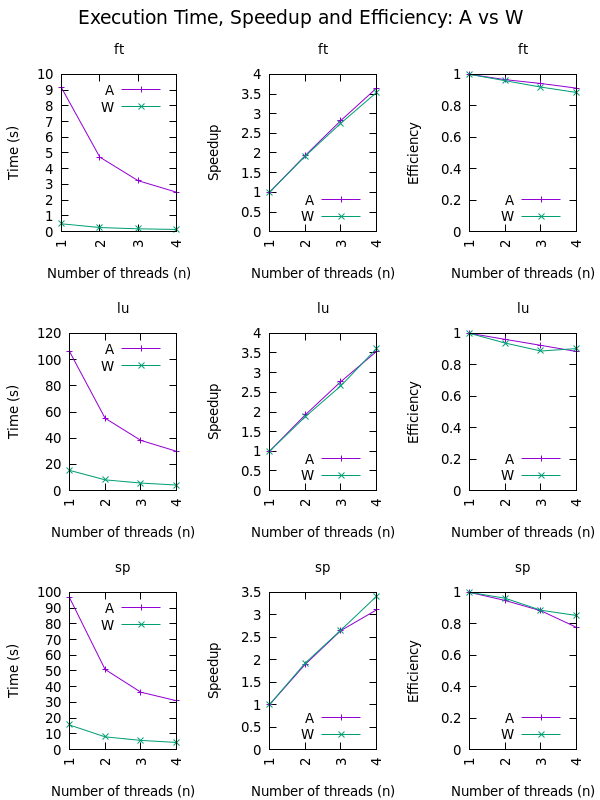
\includegraphics[width=0.9\linewidth]{ptse.png}
	\caption{Problem class A and W}
	\label{fig:aw}
\end{figure}

\newpage

\begin{figure}[h!]
	\centering
	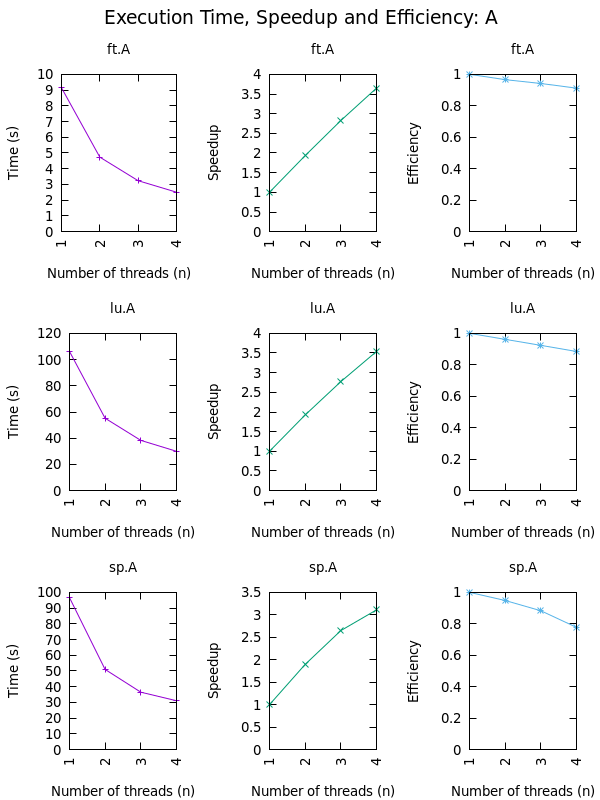
\includegraphics[width=0.9\linewidth]{A.PTSE.png}
	\caption{Problem class: A}
	\label{fig:a}
\end{figure}

\newpage

\begin{figure}[h!]
	\centering
	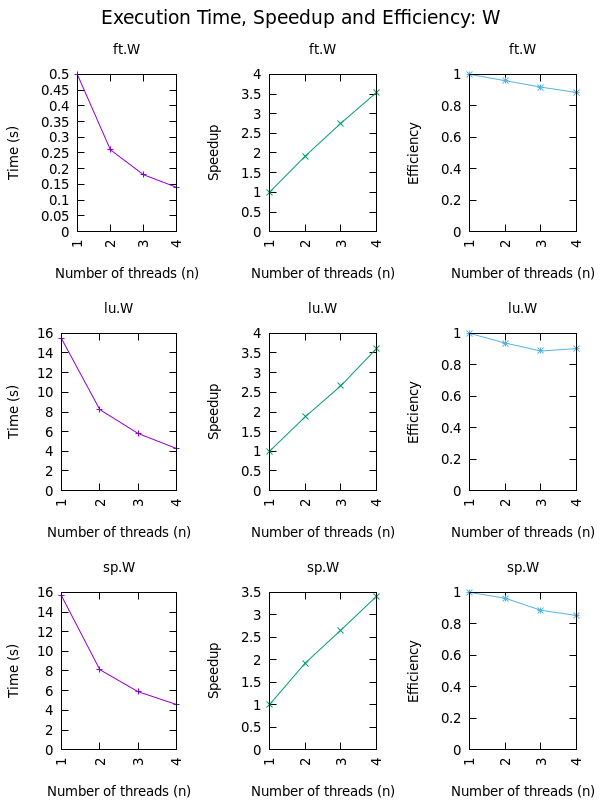
\includegraphics[width=0.9\linewidth]{W.PTSE.png}
	\caption{Problem class: W}
	\label{fig:w}
\end{figure}

\newpage

In the execution time graph, a small value is better than a larger one. In the speed-up graph, a large value is better than a smaller one. In the efficiency graph, a value close to 1 is better than another closer to 0.

In all kernels, regardless of the problem size, it seems that the execution time graph is an exponential decrease function, the speed-up graph is a linear increase function with a high slope, and the efficiency graph is a slightly pronounced linear decrease function.

The speed-up and efficiency graphs are quite similar regarding the problem size, having worse results on sp kernel with problem size A.

\begin{figure}[h!]
	\centering
	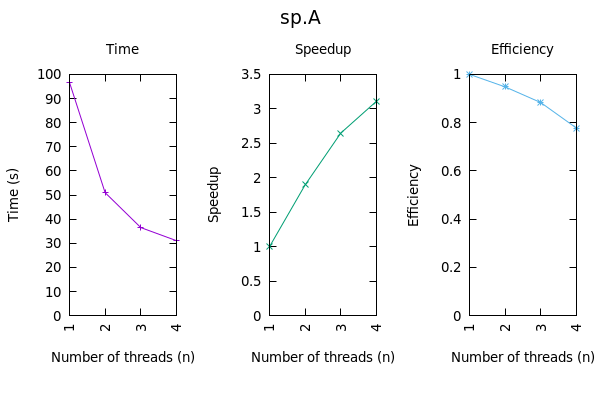
\includegraphics[width=0.9\linewidth]{sp.A.PTSE.png}
	\caption{Kernel sp class A}
	\label{fig:spa}
\end{figure}

On the other hand, it seems that the execution time graphs are quite similar between kernels, it means that sp and lu kernels have quite similar values for their execution times, and ft kernel has proportional ones.

\newpage

\section*{Question 7}

Scheduling is a method in OpenMP to distribute iterations to different threads in for loop.\footnote{\href{https://610yilingliu.github.io/2020/07/15/ScheduleinOpenMP/}{Yiling, (2020), OpenMP - Scheduling(static, dynamic, guided, runtime, auto)}}


The single-threaded execution time is the same on both kernels, about 15.5 s. However, the parallel execution with four threads has different improvement level according to the applied scheduling policy.

The sp kernel reaches higher speed-ups than lu. Almost scheduling policies applied to lu kernel reach about 3.5 of speed-up, on the other hand the lu kernel has an average speed-up value about 1,75 (excluding static scheduling), which is exactly half the speed-up value of sp kernel.

As the chunk-size increases, the speed-up deceases on both kernels. It seems that for a given chunk-size, the speed-up reaches the same level for dynamic and guided policies.

\begin{figure}[h!]
	\centering
	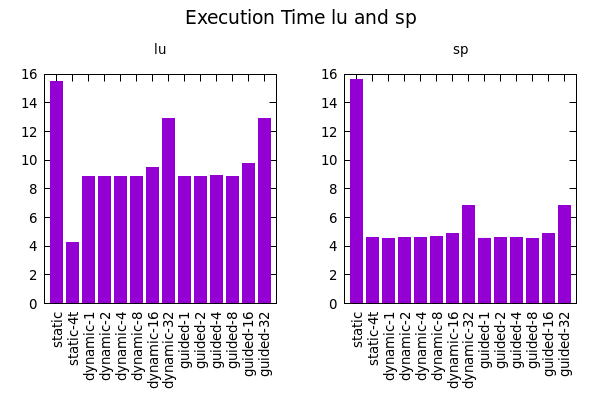
\includegraphics[width=0.8\linewidth]{scheduling_t.png}
	\caption{Execution Time lu and sp}
	\label{fig:t}
\end{figure}

\newpage

\begin{figure}[h!]
	\centering
	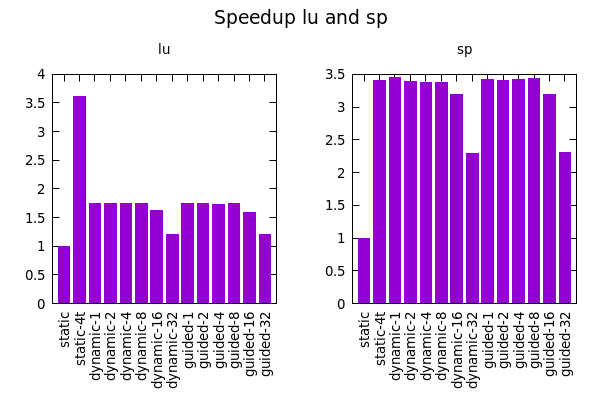
\includegraphics[width=0.8\linewidth]{scheduling_s.png}
	\caption{Speedup lu and sp}
	\label{fig:s}
\end{figure}

\begin{figure}[h!]
	\centering
	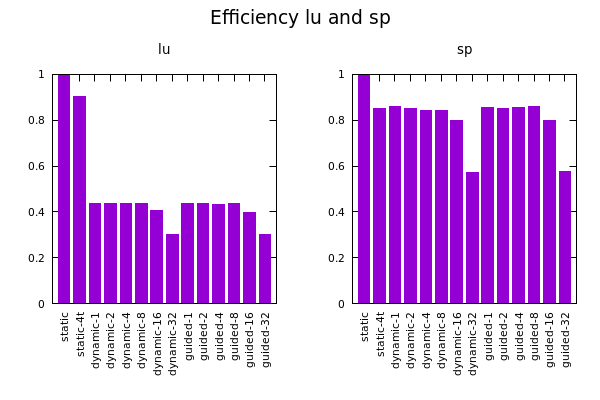
\includegraphics[width=0.8\linewidth]{scheduling_e.png}
	\caption{Efficiency lu and sp}
	\label{fig:e}
\end{figure}

\newpage

\subsection*{LU Kernel}

\begin{table}[h!]
	\centering
	\begin{tabular}{|l|c|r|r|r|}
		\hline
		scheduling & num\_threads & run\_time & speedup & efficiency \\
		\hline
		\hline
		static & 1 & 15.477 & 1 & 1 \\
		\hline
		static & 4 & 4.292 & 3.606 & 0.9015 \\
		\hline
		dynamic\_1 & 4 & 8.894 & 1.7401 & 0.435 \\
		\hline
		dynamic\_2 & 4 & 8.854 & 1.748 & 0.437 \\
		\hline
		dynamic\_4 & 4 & 8.845 & 1.7498 & 0.4374 \\
		\hline
		dynamic\_8 & 4 & 8.848 & 1.7492 & 0.4373 \\
		\hline
		dynamic\_16 & 4 & 9.51 & 1.6274 & 0.4068 \\
		\hline
		dynamic\_32 & 4 & 12.906 & 1.1992 & 0.2998 \\
		\hline
		guided\_1 & 4 & 8.838 & 1.7511 & 0.4377 \\
		\hline
		guided\_2 & 4 & 8.856 & 1.7476 & 0.4369 \\
		\hline
		guided\_4 & 4 & 8.927 & 1.7337 & 0.4334 \\
		\hline
		guided\_8 & 4 & 8.842 & 1.7503 & 0.4375 \\
		\hline
		guided\_16 & 4 & 9.747 & 1.5878 & 0.3969 \\
		\hline
		guided\_32 & 4 & 12.899 & 1.1998 & 0.2999 \\
		\hline
	\end{tabular}
	\caption{lu scheduling}
\label{tab:chunklu}
\end{table}

\begin{figure}[h!]
	\centering
	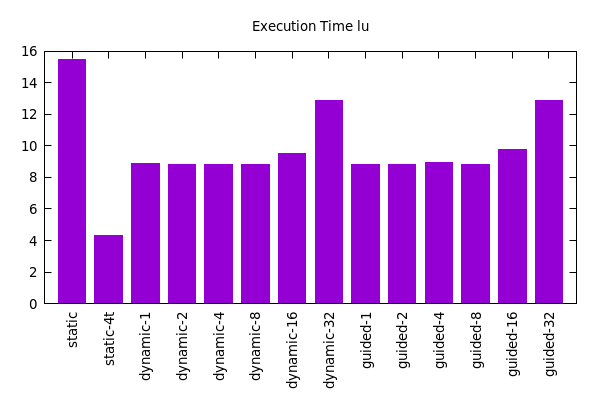
\includegraphics[width=0.7\linewidth]{lu_scheduling_t.png}
	\caption{Execution Time lu}
	\label{fig:tklu}
\end{figure}

\newpage

\subsection*{SP Kernel}

\begin{table}[h!]
	\centering
	\begin{tabular}{|l|c|r|r|r|}
		\hline
		scheduling & num\_threads & run\_time & speedup & efficiency \\
		\hline
		\hline
		static & 1 & 15.661 & 1 & 1 \\
		\hline
		static & 4 & 4.596 & 3.4075 & 0.8518 \\
		\hline
		dynamic\_1 & 4 & 4.546 & 3.445 & 0.8612 \\
		\hline
		dynamic\_2 & 4 & 4.611 & 3.3964 & 0.8491 \\
		\hline
		dynamic\_4 & 4 & 4.642 & 3.3737 & 0.8434 \\
		\hline
		dynamic\_8 & 4 & 4.647 & 3.3701 & 0.8425 \\
		\hline
		dynamic\_16 & 4 & 4.906 & 3.1922 & 0.798 \\
		\hline
		dynamic\_32 & 4 & 6.825 & 2.2946 & 0.5736 \\
		\hline
		guided\_1 & 4 & 4.575 & 3.4231 & 0.8557 \\
		\hline
		guided\_2 & 4 & 4.607 & 3.3993 & 0.8498 \\
		\hline
		guided\_4 & 4 & 4.579 & 3.4201 & 0.855 \\
		\hline
		guided\_8 & 4 & 4.558 & 3.4359 & 0.8589 \\
		\hline
		guided\_16 & 4 & 4.911 & 3.1889 & 0.7972 \\
		\hline
		guided\_32 & 4 & 6.813 & 2.2986 & 0.5746 \\
		\hline
	\end{tabular}
	\caption{sp scheduling}
\label{tab:chunksp}
\end{table}

\begin{figure}[h!]
	\centering
	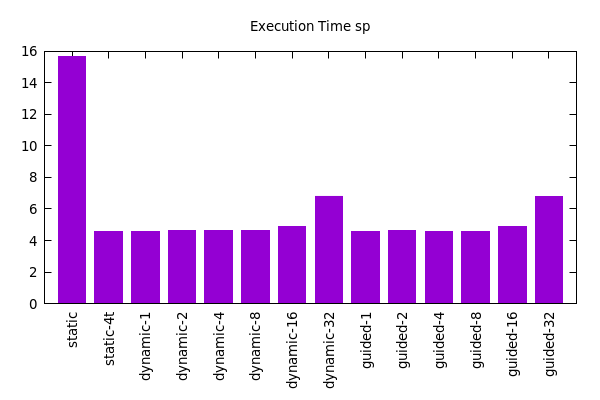
\includegraphics[width=0.7\linewidth]{sp_scheduling_t.png}
	\caption{Execution Time sp}
	\label{fig:tksp}
\end{figure}

\newpage

\section{List of commands}

\begin{figure}[h!]
	\begin{minted}{shell}
# queue jobs
qsub -N hello_omp_v1_3 hello_omp_v1.sge
qsub -N hello_omp_v2_3 -v OMP_NUM_THREADS='3' hello_omp_v2.sge
qsub -N hello_omp_v2_2 -v OMP_NUM_THREADS='2' hello_omp_v2.sge
qsub -N hello_omp_v2_1 -v OMP_NUM_THREADS='1' hello_omp_v2.sge
	\end{minted}
\caption{Warm-up Activity}\label{code:wa}
\end{figure}

\begin{figure}[h!]
	\begin{minted}{shell}
# queue jobs
./queue.sh -s sv -p sv_omp -n 1000000000 | sh

# get dat and png files from csv files
./sumarize_sv.sh
	\end{minted}
\caption{Question 1}\label{code:q1}
\end{figure}

\begin{figure}[h!]
	\begin{minted}{shell}
# queue jobs
./queue_mm.sh | sh

# get dat and png files from csv files
./sumarize_mm.sh
	\end{minted}
\caption{Question 2}\label{code:q2}
\end{figure}

\begin{figure}[h!]
	\begin{minted}{shell}
# queue jobs
./queue_flops.sh -n flops | sh
./queue_flops.sh -n flops2 | sh
	\end{minted}
\caption{Question 3}\label{code:q3}
\end{figure}

\newpage

\begin{figure}[h!]
	\begin{minted}{shell}
# get counter list
qsub papi_avail.sge

# queue jobs
./queue_all_counters.sh | sh

# get csv files
./sumarize_counters.sh
	\end{minted}
\caption{Question 5}\label{code:q5}
\end{figure}

\begin{figure}[h!]
	\begin{minted}{shell}
# queue jobs
./queue_npb.sh | sh

# get csv, dat and png files
./sumarize_npb.sh
	\end{minted}
\caption{Question 6}\label{code:q6}
\end{figure}

\begin{figure}[h!]
	\begin{minted}{shell}
# get binaries
./build_scheduling.sh

# queue jobs
./queue_scheduling.sh | sh

# csv files
./sumarize_scheduling.sh
	\end{minted}
	\caption{Question 7}\label{code:q7}
\end{figure}

\end{document}
